\subsection{Evaluating Quality of Financial Reports}

\begin{definition}{\color{white}space}
\begin{enumerate}[label=\roman*.]
\setlength{\itemsep}{0pt}
\item \hlt{Earnings Quality}: high-quality earnings quality refers to a high level of earnings and is sustainable. High-quality earnings increase the value of a company more than low-quality earnings.
\item \hlt{Reporting Quality}: assessment of information disclosed in the financial reports. Low-quality reporting impedes assessment, while high-quality earnings enable it.
\end{enumerate}
\end{definition}

\begin{figure}[H]
\centering
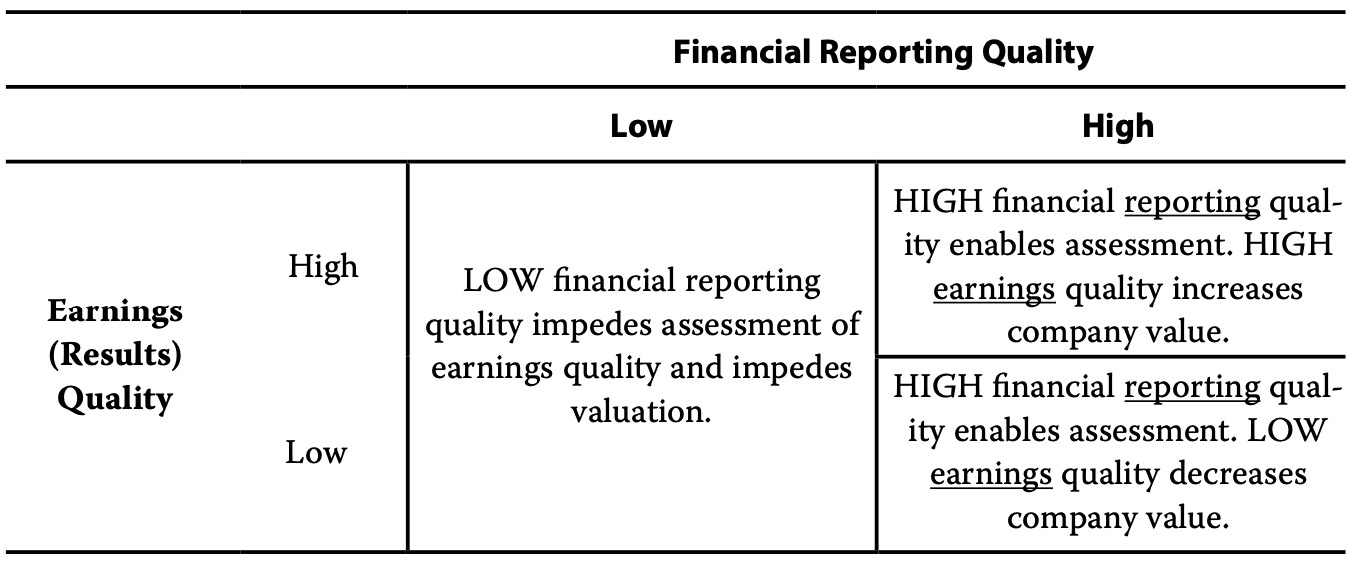
\includegraphics[scale=0.5]{fsa/reportvsearningquality}
\caption{Relationship between reporting quality and earnings quality.}
\end{figure}

\begin{figure}[H]
\centering
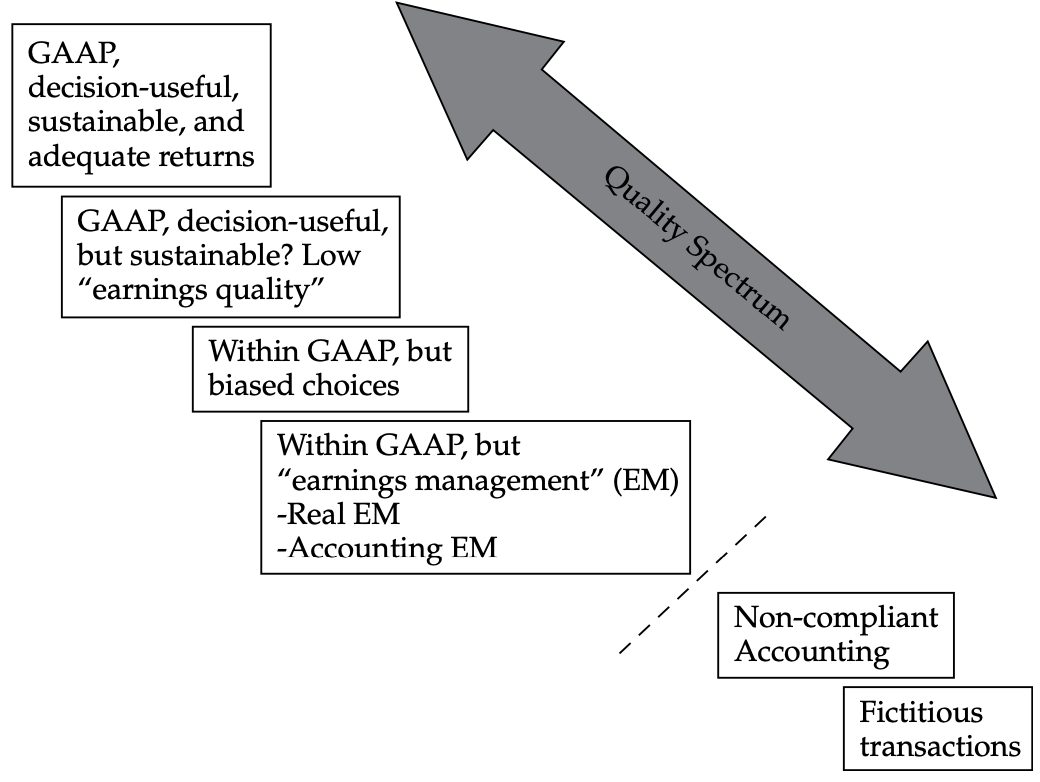
\includegraphics[scale=0.6]{fsa/qualityspectrum}
\caption{Quality spectrum of financial reports.}
\end{figure}

\begin{remark} \hlt{Biased Accounting}\\
Biased accounting result in financial reports that don’t faithfully represent economic phenomena. May be made in context of reported amounts and presented info.\\
Earnings management include smoothing of earnings to understate earnings volatility. Volatility decreased by understating earnings in well performing periods, overstated in struggling periods.
\end{remark}

\newpage 

\begin{landscape}

\begin{flushleft}
Accounting Warning Signs\\
\begin{tabularx}{\hsize}{p{20em}|p{22em}|p{28em}}
\hline
\rowcolor{gray!30}
Potential Issues & Possible Actions \& Choices & Warning Signs \\
\hline
\xxx Overstatement or non-sustainability of operating income, net income
\xxx Overstated or accelerated revenue recognition
\xxx Understated expenses
\xxx Misclassification of revenue, gains, expenses, or losses
&
\xxx Contingent sales with right of return, “channel stuffing” (the practice of inducing customers to order products they would otherwise not order or order at a later date through generous terms), “bill and hold” sales (encouraging customers to order goods and retain them on seller’s premises)
\xxx Fictitious (fraudulent) revenue
\xxx Capitalising expenditures as assets
\xxx Classifying non-operating income or gains as part of operations
\xxx Classifying ordinary expenses as non-recurring or non-operating
\xxx Reporting gains through net income and losses through other comprehensive income
&
\xxx Growth in revenue higher than that of industry or peers
\xxx Increases in discounts to and returns from customers
\xxx Higher growth rate in receivables than revenue
\xxx Large proportion of revenue in final quarter of year for a non-seasonal business
\xxx Cash flow from operations is much lower than operating income
\xxx Inconsistency over time in the items included in operating revenues and operating expenses
\xxx Increases in operating margin
\xxx Aggressive accounting assumptions, i.e, long, depreciable lives
\xxx Losses in non-operating income or other comprehensive income and gains in operating income or net income
\xxx Compensation largely tied to financial results \\
\hline
\xxx Misstatement of balance sheet items (may affect income statement)
\xxx Over- or understatement of assets
\xxx Over- or understatement of liabilities
\xxx Misclassification of assets and/or liabilities
&
\xxx Choice of models and model inputs to measure fair value
\xxx Classification from current to non-current
\xxx Over- or understating reserves and allowances
\xxx Understating identifiable assets and overstating goodwill &
\xxx Models and model inputs that bias fair value measures
\xxx Inconsistency in model inputs when measuring fair value of assets com- pared with that of liabilities
\xxx Typical current assets, such as accounts receivable and inventory, included in non-current assets
\xxx Allowances and reserves that fluctuate over time or are not comparable with peers
\xxx High goodwill value relative to total assets
\xxx Use of special purpose vehicles
\xxx Large changes in deferred tax assets and liabilities
\xxx Significant off-balance-sheet liabilities
\\
\hline
\xxx Overstatement of cash flow from operations
&
\xxx Managing activities to affect cash flow from operations
\xxx Misclassifying cash flows to positively affect cash flow from operations
&
\xxx Increase in accounts payable and decrease in accounts receivable and inventory
\xxx Capitalised expenditures in investing activities
\xxx Sales and leaseback
\xxx Increases in bank overdrafts \\
\hline
\end{tabularx}
\end{flushleft}

\end{landscape}

\newpage

\begin{remark} \hlt{Acquisition Method Accounting}
\begin{enumerate}[label=\roman*.]
\setlength{\itemsep}{0pt}
\item Companies with decreasing cash-generating ability may acquire other companies to increase CFO; payment reported in CFI (if in cash), or not in cash flow statements if paid with equity. Consolidated CFO include CF from acquired company, concealing the acquirer’s own CF issues, providing one-time boost to CFO.
\item Acquirers making acquisition with equity may manipulate reported earnings prior to acquisition to inflate value of shares. Acquirer may also manipulate earnings upward after acquisition to positively influence opinion on the acquisition.
\item Acquisitions may conceal previous accounting misstatements, by acquiring company that reduce comparability and consistency of financial statements, i.e., companies with less public info, less similar ops.
\item Company may capitalise goodwill indefinitely, hence postpone recognition of an uneconomic acquisition. 
\end{enumerate}
\end{remark}

\begin{remark} \hlt{Compliant, but not Economic Reality}\\
Investor to adjust reported information to better reflect view on economic reality; if not possible as relevant data are not disclosed, may make qualitative assessment.
\begin{enumerate}[label=\roman*.]
\setlength{\itemsep}{0pt}
\item On restructuring charge, impairment charge, or combination of two, to consider whether similar events should be factored into estimated of permanent earnings (hence normalised by spreading current restructuring/impairment charges over past and current periods), or regarded as one-off items.
\item Revisions to ongoing estimates, such as remaining economic lives of assets, may question if earlier change in estimate would have been more appropriate.
\item Sudden increase to allowance and reserves, may question if prior estimates resulted in overstatements of prior period earnings.
\item Large accruals for losses (i.e., environmental or litigation-related) suggest that prior periods earnings may be overstated due to failure to accrue losses earlier.
\item Significant order backlogs (disclosed in management commentary) may be used to adjust reported amounts and to prepare forecasts.
\end{enumerate}
Also, to judge whether an item presented in OCI should be included in analysis as net income:
\begin{enumerate}[label=\roman*.]
\setlength{\itemsep}{0pt}
\item unrealised holding gains and losses on certain investments in equity securities,
\item unrealised holding gains (and subsequent losses) on items of property and equipment for which the 'revaluation option' is elected (IFRS only),
\item effects on owners’ equity resulting from the translation of the foreign currency-denominated financial statements of a foreign operation to the reporting currency of the consolidated entity,
\item certain changes to net pension liability or asset, and
\item gains and losses on derivative financial instruments (and certain foreign currency-denominated non-derivative financial instruments) accounted for as a hedge of future cash flows.
\end{enumerate}
\end{remark}

\begin{method} \hlt{General Steps to Evaluate Quality of Financial Reports}
\begin{enumerate}[label=\arabic*.]
\setlength{\itemsep}{0pt}
\item Develop understanding of company and its industry (economic activities, accounting principles), and assess if the accounting treatment is appropriate.
\item Evaluate company management, if any. Incentives to misreport. Review disclosures on compensation and insider transactions, related-party transactions.
\item Identify significant account areas which management judgment or unusual accounting rule is significant determinant of reported financial performance.
\item Make comparisons:
\begin{enumerate}[label=\roman*.]
\setlength{\itemsep}{0pt}
\item Compare firm financial statement and significant disclosures in current year report with financial statements and significant disclosures in prior year report. Check for major differences in line items or in key disclosures (i.e., risk disclosures, segment disclosures, classification of specific expense, revenue items). Check if reasons for changes are apparent.
\item Compare firm accounting policies with closest competitors for significant differences, and direction effect of the differences.
\item Use ratio analysis, compare firm performance with closest competitors.
\end{enumerate}
\item Check for warning sings of possible issues with quality of financial report:
\begin{enumerate}[label=\roman*.]
\setlength{\itemsep}{0pt}
\item Declining receivables turnover could suggest some revenues are fictitious, or recorded prematurely, or allowance for doubtful accounts is insufficient.
\item Declining inventory turnover could suggest obsolescence problems
\item Net income greater than cash provided by operations could suggest aggressive accrual accounting policies have shifted current expenses to later periods
\end{enumerate}
\item Firms operating in multiple segments by geography or product (MNCs), consider if inventory, sales, and expenses have shifted to make it appear that the firm is positively exposed to a geographic region or product segment that investment community considers to be a desirable growth area. This shift may be occurring if the segment is showing strong performance while consolidated results remain static or worsen.
\item Use appropriate quantitative tools to assess likelihood of misreporting
\end{enumerate}
\end{method}

\subsubsection{Earnings Quality Analysis}

\begin{definition} \hlt{Beneish Model}\\
Probit regression model that estimate probability of earnings manipulation using eight independent variables.\\
M-score determines the probability of earnings manipulation. Higher values indicate higher probabilities.
\begin{align}
\text{M-Score} = &-4.84 + 0.920(\text{DSR}) + 0.528(\text{GMI}) + 0.404(\text{AQI}) + 0.892(\text{SGI}) \nonumber \\
&+ 0.115(\text{DEPI}) - 0.172(\text{SGAI}) + 4.679(\text{Accruals}) - 0.327(\text{LEVI}) \nonumber
\end{align}
where
\begin{enumerate}[label=\roman*.]
\setlength{\itemsep}{0pt}
\item DSR (Days Sales Receivable Index): changes in relationship between receivables and sales could indicate inappropriate revenue recognition.
\begin{equation}
\text{DSR} = \left(\frac{\text{Receivables}_t}{\text{Sales}_t} \right) \div \left(\frac{\text{Receivables}_{t-1}}{\text{Sales}_{t-1}} \right) \nonumber
\end{equation}
\item GMI (Gross Margin Index): deterioration in margins could predispose companies to manipulate earnings.
\begin{equation}
\text{GMI} = \frac{\text{Gross Margin}_{t-1}}{\text{Gross Margin}_{t}} \nonumber
\end{equation}
\item AQI (Asset Equality Index): change in percentage of assets other than in PPE and CA could indicate excessive expenditure capitalisation.
\begin{equation}
\text{AQI} = \left[1- \frac{(\text{PPE}_t + \text{CA}_t)}{\text{TA}_t} \right] \div \left[1- \frac{(\text{PPE}_{t-1} + \text{CA}_{t-1})}{\text{TA}_{t-1}} \right] \nonumber
\end{equation}
where PPE is property, plant, and equipment; CA is current assets; and TA is total assets.
\item SGA (Sales Growth Index): managing perception of continuing growth and capital needs from actual growth could predispose companies to manipulate sales and earnings.
\begin{equation}
\text{SGA} = \frac{\text{Sales}_{t}}{\text{Sales}_{t-1}} \nonumber
\end{equation}
\item DEPI (Depreciation Index): declining depreciation rates could indicate understated depreciation as a means of manipulating earnings.
\begin{align}
\text{DEPI} &= \frac{\text{Depreciation Rate}_{t-1}}{\text{Depreciation Rate}_{t}} \nonumber \\
\text{Depreciation Rate} &= \frac{\text{Depreciation}}{\text{Depreciation} + \text{PPE}} \nonumber
\end{align}
\item SGAI (Sales, General, and Administrative Expenses Index): increase in fixed SGA expenses suggests decreasing administrative \& marketing efficiency, which could predispose companies to manipulate earnings.
\begin{equation}
\text{SGAI} = \left(\frac{\text{SGA}_t}{\text{Sales}_t} \right) \div \left(\frac{\text{SGA}_{t-1}}{\text{Sales}_{t-1}} \right) \nonumber
\end{equation}
\item Accruals: higher accruals can indicate earnings manipulation.
\begin{equation}
\text{Accruals} = \frac{\text{Income Before Extraordinary Items} - \text{Cash from Operations}}{\text{Total Assets}} \nonumber
\end{equation}
\item LEVI (Leverage Index): increasing leverage could predispose companies to manipulate earnings.
\begin{equation}
\text{LEVI} = \frac{\text{Leverage}_t}{\text{Leverage}_{t-1}} \nonumber
\end{equation}
\end{enumerate}
M-score is a normally distributed random variable with mean $0$ and standard deviation $1$.\\
Probability of earnings manipulation is then cumulative probability for standard normal distribution based on the M-score. Likely cutoff is probability of earnings manipulation of $3.8\%$ (M-score $> -1.78$).
\end{definition}

\begin{remark} \hlt{Limitations of Beneish Model}\\
Beneish model relies on accounting data, which may not reflect economic reality.\\
Deeper analysis of underlying relationships may be warranted to get a clearer picture.\\
As managers become aware of the use of specific quantitative tools, they may begin to game the measures used. 
\end{remark}

\begin{remark} \hlt{Other Quantitative Models}\\
Other quantitative models may include variables such as accruals quality, deferred taxes, auditor change, market-to-book value, whether company is publicly listed and traded; growth rate differences between financial and non-financial variables (i.e., number of patents, employees, products); aspects of corporate governance and incentive comp.
\end{remark}

\begin{method} \hlt{Altman Model}\\
Model is able to assess the probability that a firm will file for bankruptcy.\\
Model relies on discriminant analysis to generate Z-score with five variables:
\begin{align}
\frac{\text{Net Working Capital}}{\text{Total Assets}}, \ \frac{\text{Retained Earnings}}{\text{Total Assets}}, \ \frac{\text{Operating Profit}}{\text{Total Assets}}, \  \frac{\text{Market Value of Equity}}{\text{Book Value of Liabilities}}, \ \frac{\text{Sales}}{\text{Total Assets}} \nonumber
\end{align}
Each variable is positively related to the Z-score, and a higher Z-score is better (less likelihood of bankruptcy).\\
It is a single-period static model and does not capture change in key variables over time. Additionally, similar to the Beneish model, Altman’s model mostly uses accounting data. 
\end{method}

\begin{remark} \hlt{Indicators of Earnings Quality}\\
Recurring earnings, earnings persistence and related measures of accruals, beating benchmarks, and after-the-fact confirmations of poor-quality earnings, such as enforcement actions and restatements.
\end{remark}

\begin{definition} \hlt{Non-Recurring Earnings}\\
Earnings from subsidiaries selected for disposal; one-off asset sales; one-off litigation or tax settlements.\\
Earnings with high proportion of non-recurring items less likely to be sustainable, hence considered lower quality.\\
Companies may disclose pro forma (adjusted) income that exclude non-recurring items; there is reconciliation between pro-forma and reported income.
\end{definition}

\begin{definition} \hlt{Classification Shifting}\\
Accomplished by re-classifying normal expenses to special items, or shift operating expenses to income-decreasing discontinued operations. \\
Does not affect total net income, can inflate the amount reported as recurring or core earnings.\\
Be wary of large special items or when the company is reporting unusually large operating income for a period. 
\end{definition}